% COSC 431 — Deliverable 1 submission document
% Build:  cd docs/latex && tectonic deliverable1.tex
% Appendices are generated from the repo's data files by:
%         python scripts/make_latex_appendices.py
\documentclass[11pt]{article}

\usepackage[margin=1in]{geometry}
\usepackage[T1]{fontenc}
\usepackage{lmodern}
\usepackage{amsmath,amssymb}
\usepackage{booktabs}
\usepackage{longtable}
\usepackage{listings}
\usepackage{xcolor}
\usepackage{tikz}
\usepackage{enumitem}
\usepackage[colorlinks=true,linkcolor=blue!50!black,urlcolor=blue!50!black]{hyperref}
\usetikzlibrary{positioning,arrows.meta,shapes.geometric}

\definecolor{codebg}{gray}{0.96}
\definecolor{kw}{rgb}{0.0,0.3,0.6}
\lstdefinestyle{sql}{
  language=SQL,
  basicstyle=\ttfamily\footnotesize,
  keywordstyle=\color{kw}\bfseries,
  backgroundcolor=\color{codebg},
  breaklines=true,
  breakatwhitespace=false,
  columns=fullflexible,
  frame=single,
  framerule=0pt,
  xleftmargin=6pt,
  framexleftmargin=6pt,
  showstringspaces=false,
  morekeywords={EXCEPT,EXISTS,HAVING,LIMIT,DISTINCT}
}
\lstset{style=sql}

% Relational algebra shorthands
\newcommand{\proj}[1]{\pi_{#1}}
\newcommand{\sel}[1]{\sigma_{#1}}
\newcommand{\agg}[1]{\gamma_{#1}}
\newcommand{\jn}{\bowtie}

\title{\textbf{AI Query Check}\\[0.3em]
\large Evaluating the Correctness, Security, and Performance of LLM-Generated SQL\\[0.6em]
\normalsize Deliverable 1: Benchmark Construction}

\author{%
Jelani Denmark (pipeline) \and
Joshua Sanders (question set) \and
Isaiah Washington (formal methods \& security) \and
Maxwell Amakor (schema \& performance)%
}
\date{COSC 431 --- Database Management \\ \today \\[0.8em]
\normalsize Project repository: \url{https://github.com/jd702/cosc431-ai-query-check}}

\begin{document}
\maketitle

\begin{abstract}
\noindent
This deliverable builds the benchmark that Deliverable 2 will use to evaluate LLM-generated SQL.
We selected the Chinook digital-media-store schema, adapted 20 natural-language questions with
expert-verified gold SQL from the Spider benchmark, executed and verified every gold answer
against a local SQLite database, expressed five of the queries in relational algebra and tuple
relational calculus, and constructed a deliberately denormalized schema variant for the
performance comparison. All 20 queries execute without error and return non-empty results.
\end{abstract}

\section{Submission checklist}

\begin{center}
\begin{tabular}{@{}llp{6.1cm}@{}}
\toprule
\textbf{Required item} & \textbf{Section} & \textbf{File in repository} \\
\midrule
Normalized schema (DDL)            & App.~\ref{app:ddl} & \texttt{sql/normalized\_schema.sql} \\
Denormalized variant + explanation & \S\ref{sec:denorm} & \texttt{sql/denormalized\_schema.sql} \\
20 questions + verified gold SQL   & App.~\ref{app:questions} & \texttt{data/questions.json} \\
\quad and their result sets        & App.~\ref{app:questions} & \texttt{data/gold\_results.json} \\
3--5 queries in relational algebra & \S\ref{sec:algebra} & \texttt{docs/relational\_algebra.md} \\
Write-up                           & \S\ref{sec:schema}--\ref{sec:limits} & \texttt{docs/deliverable1\_writeup.md} \\
\bottomrule
\end{tabular}
\end{center}

\noindent
Every artifact is reproducible from the repository with a single command,
\texttt{python scripts/setup\_db.py}, which downloads the Chinook SQL script, builds both
database variants, and regenerates the DDL in Appendix~\ref{app:ddl}.

\section{Schema choice}\label{sec:schema}

We chose \textbf{Chinook}, a digital media store, over Sakila. It is the smaller of the two
options (11 tables against Sakila's 16), which let us spend our effort on the evaluation rather
than on learning an unfamiliar schema, and it ships as a single SQLite script, so every team
member can rebuild a byte-identical database. Chinook is also represented in Spider as
\texttt{chinook\_1}, so the questions we adapted were written against the same table and column
names we query, which kept adaptations minimal.

\begin{center}
\begin{tabular}{@{}lrl@{}}
\toprule
\textbf{Table} & \textbf{Rows} & \textbf{Role} \\
\midrule
Artist        & 275   & Recording artists \\
Album         & 347   & Albums, each belonging to one artist \\
Track         & 3{,}503 & Individual tracks; the largest base table \\
Genre         & 25    & Track genres \\
MediaType     & 5     & Encoding formats \\
Playlist      & 18    & Named playlists \\
PlaylistTrack & 8{,}715 & Many-to-many bridge, playlists to tracks \\
Customer      & 59    & Customers, each assigned a support representative \\
Employee      & 8     & Staff, with a self-referencing \texttt{ReportsTo} hierarchy \\
Invoice       & 412   & Customer invoices \\
InvoiceLine   & 2{,}240 & Line items on each invoice \\
\bottomrule
\end{tabular}
\end{center}

The relationships give us the structural variety the project needs: simple one-to-many chains
(Artist $\rightarrow$ Album $\rightarrow$ Track), a many-to-many bridge (PlaylistTrack), a
self-referencing hierarchy (\texttt{Employee.ReportsTo}), and nullable foreign keys
(\texttt{Track.AlbumId}, \texttt{Track.GenreId}, \texttt{Customer.SupportRepId}) that make join
choice consequential. The Customer $\rightarrow$ Invoice $\rightarrow$ InvoiceLine
$\rightarrow$ Track path is four tables deep, which is what makes the denormalization and
indexing comparisons in Deliverable 2 meaningful.

Chinook as distributed is already in 3NF, so no normalization work was required to reach it.
That is why this deliverable's normalization work runs in the opposite direction: we deliberately
break 3NF to construct the denormalized variant in \S\ref{sec:denorm}. Chinook also ships 11
foreign-key indexes of its own (named \texttt{IFK\_*}), a detail that materially affects the
Deliverable 2 performance method (\S\ref{sec:limits}).

\subsection{ER diagram}

\begin{center}
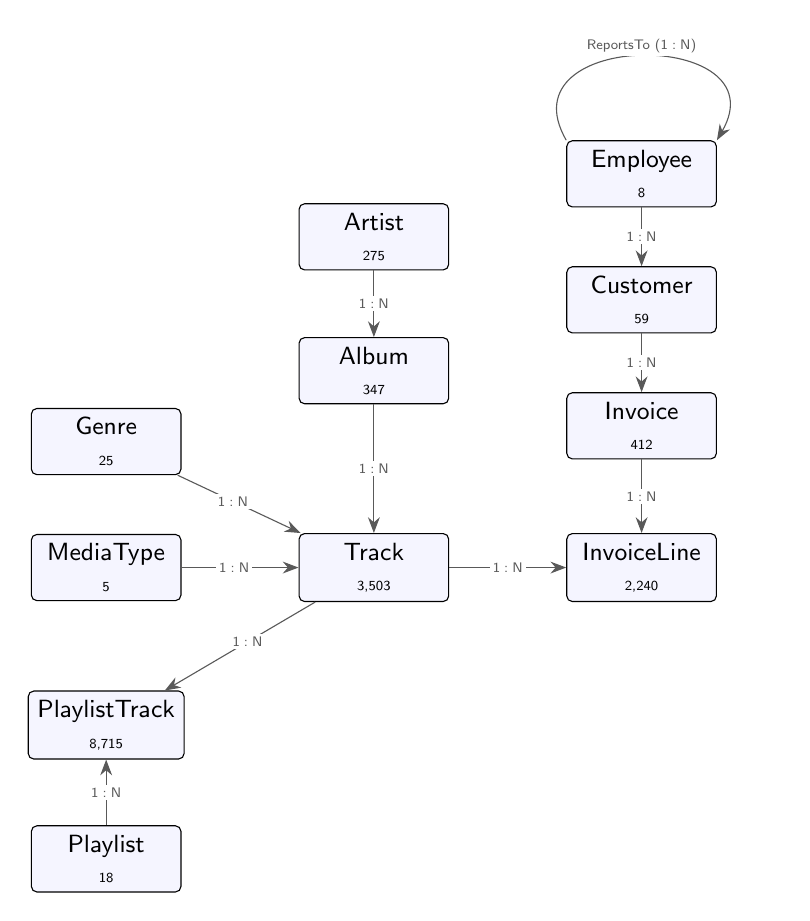
\begin{tikzpicture}[
  ent/.style={draw, rounded corners=2pt, align=center, font=\small\sffamily,
              minimum height=7mm, minimum width=19mm, fill=blue!4},
  rel/.style={-{Stealth[length=2mm]}, gray!70!black, thin},
  lbl/.style={font=\tiny\sffamily, inner sep=1pt, fill=white}
]
% left chain
\node[ent] (artist)   at (0,5.2)   {Artist\\\tiny 275};
\node[ent] (album)    at (0,3.5)   {Album\\\tiny 347};
\node[ent] (track)    at (0,1.0)   {Track\\\tiny 3,503};
% left-side lookups
\node[ent] (genre)    at (-3.4,2.6) {Genre\\\tiny 25};
\node[ent] (media)    at (-3.4,1.0) {MediaType\\\tiny 5};
% playlists
\node[ent] (pltrack)  at (-3.4,-1.0) {PlaylistTrack\\\tiny 8,715};
\node[ent] (playlist) at (-3.4,-2.7) {Playlist\\\tiny 18};
% sales chain
\node[ent] (invline)  at (3.4,1.0)  {InvoiceLine\\\tiny 2,240};
\node[ent] (invoice)  at (3.4,2.8)  {Invoice\\\tiny 412};
\node[ent] (customer) at (3.4,4.4)  {Customer\\\tiny 59};
\node[ent] (employee) at (3.4,6.0)  {Employee\\\tiny 8};

\draw[rel] (artist)   -- node[lbl,pos=0.5]{1\;:\;N} (album);
\draw[rel] (album)    -- node[lbl,pos=0.5]{1\;:\;N} (track);
\draw[rel] (genre)    -- node[lbl,pos=0.45]{1\;:\;N} (track);
\draw[rel] (media)    -- node[lbl,pos=0.45]{1\;:\;N} (track);
\draw[rel] (track)    -- node[lbl,pos=0.45]{1\;:\;N} (pltrack);
\draw[rel] (playlist) -- node[lbl,pos=0.5]{1\;:\;N} (pltrack);
\draw[rel] (track)    -- node[lbl,pos=0.5]{1\;:\;N} (invline);
\draw[rel] (invoice)  -- node[lbl,pos=0.5]{1\;:\;N} (invline);
\draw[rel] (customer) -- node[lbl,pos=0.5]{1\;:\;N} (invoice);
\draw[rel] (employee) -- node[lbl,pos=0.5]{1\;:\;N} (customer);
\draw[rel] (employee.north west) to[out=120,in=60,looseness=2.2]
      node[lbl,above,pos=0.5]{ReportsTo (1\;:\;N)} (employee.north east);
\end{tikzpicture}
\end{center}

\noindent
Arrows point from the ``one'' side to the ``many'' side. \texttt{Track.AlbumId},
\texttt{Track.GenreId} and \texttt{Customer.SupportRepId} are nullable; all other foreign keys
are mandatory. Full attribute lists are in Appendix~\ref{app:ddl}.

\section{Question sources and adaptations}\label{sec:questions}

All 20 question/gold-SQL pairs were drawn from the Spider benchmark's \texttt{chinook\_1}
database (\texttt{train\_spider.json}), not invented from scratch. We favored easy and medium
difficulty as the project guide recommends, and selected for a mix of query shapes.

\begin{center}
\begin{tabular}{@{}lr@{\qquad}lr@{}}
\toprule
\textbf{Difficulty} & \textbf{Count} & \textbf{Query shape} & \textbf{Count} \\
\midrule
Easy   & 6  & Single-table lookup       & 7 \\
Medium & 14 & Join (2--3 tables)        & 7 \\
Hard   & 0  & Aggregation (\textsc{count}/\textsc{sum}/\textsc{avg}, \textsc{group by}) & 5 \\
       &    & Subquery                  & 1 \\
\midrule
\textbf{Total} & \textbf{20} & \textbf{Total} & \textbf{20} \\
\bottomrule
\end{tabular}
\end{center}

Nine questions required adaptation. Three were changed in response to an internal review that
found the question wording and the gold SQL disagreed --- a mismatch that would have penalized a
model for answering the question as written.

\begin{center}
\begin{longtable}{@{}llp{9.2cm}@{}}
\toprule
\textbf{ID} & \textbf{Spider index} & \textbf{Change made} \\
\midrule
\endfirsthead
\toprule
\textbf{ID} & \textbf{Spider index} & \textbf{Change made} \\
\midrule
\endhead
Q05 & 864 & Reworded to ``List the phone numbers of all employees'' so the question matches the
            gold SQL, which projects only \texttt{Phone}. \\
Q08 & 822 & Adapted to our table and column names. \\
Q11 & 849 & None needed; Chinook uses identical table and column names. \\
Q12 & 870 & Corrected the original gold SQL, which selected the \emph{customer's} first name
            instead of the \emph{employee's} and was grouped incorrectly. \\
Q13 & 837 & Tightened the \textsc{group by} to include both \texttt{MediaTypeId} and
            \texttt{Name}. \\
Q15 & 840 & Added \texttt{Title} to the \textsc{group by} so the album title is grouped with its
            id. \\
Q16 & 872 & Changed \textsc{inner join} to \textsc{left join} so employees serving zero
            customers are not excluded, and clarified the question to say so. \\
Q17 & 888 & Changed \textsc{not in} to \textsc{not exists}, avoiding SQL's three-valued-logic
            behavior when the inner result contains \textsc{null}. \\
Q20 & 888 & Adapted the question and SQL to our schema. \\
\bottomrule
\end{longtable}
\end{center}

Typographical errors present in the original Spider wording (for example ``unite price'',
``do nout have'') were deliberately left in place, to keep the questions faithful to the source
dataset rather than silently improving the prompts the models receive.

\subsection{Verification method}

\begin{enumerate}[leftmargin=*,topsep=2pt,itemsep=2pt]
  \item \texttt{notebooks/01\_build\_benchmark.ipynb} executes every gold query against
        \texttt{data/chinook.db} and writes the result sets to \texttt{data/gold\_results.json}.
  \item The notebook asserts that the set contains 15--20 questions, that IDs are unique, and
        that at least one question is a subquery.
  \item Every result was reviewed by a team member other than the author of its SQL.
  \item Selected answers were cross-checked independently against the raw data. For example,
        Q13's ``least common media type'' returns \emph{Purchased AAC audio file} (7 tracks,
        fewer than \emph{AAC audio file}'s 11), and Q17's count of artists without an album
        returns 71 (275 artists, of which 204 have at least one album).
\end{enumerate}

\noindent
All 20 queries execute with no SQL errors and no empty result sets.

\section{Formal query notation}\label{sec:algebra}

Five queries are expressed below in relational algebra, one additionally in tuple relational
calculus. Each uses the verified gold SQL verbatim, so the identifiers match
Appendix~\ref{app:questions}. Operators: $\sigma$ selection, $\pi$ projection, $\jn$ join,
$\gamma$ grouping and aggregation, $-$ set difference.

\subsection*{Q06 --- Invoice dates for the customer Astrid Gruber}

\begin{lstlisting}
SELECT T2.InvoiceDate FROM CUSTOMER AS T1
JOIN INVOICE AS T2 ON T1.CustomerId = T2.CustomerId
WHERE T1.FirstName = 'Astrid' AND T1.LastName = 'Gruber'
\end{lstlisting}

\[
\proj{InvoiceDate}\bigl(\sel{FirstName='Astrid'\,\wedge\,LastName='Gruber'}(
  \text{Customer} \jn_{\text{CustomerId}} \text{Invoice})\bigr)
\]

An equivalent form pushes the selection below the join, which is exactly the rewrite a query
optimizer performs:
\[
\proj{InvoiceDate}\bigl(
  \sel{FirstName='Astrid'\,\wedge\,LastName='Gruber'}(\text{Customer})
  \jn_{\text{CustomerId}} \text{Invoice}\bigr)
\]

\textbf{Comparison.} The algebra makes evaluation \emph{order} explicit: the first form filters
after materializing the join, the second filters first. Both denote the same relation, which is
precisely why the rewrite is legal. The SQL states no order at all; it declares the result and
delegates the plan to the engine, and \texttt{EXPLAIN QUERY PLAN} confirms SQLite chooses the
second form. Conversely, the algebra requires an explicit theta-join condition
$\jn_{\text{CustomerId}}$, because a natural join would silently equate every identically named
column the two relations share --- a hazard the SQL's explicit \textsc{on} clause avoids.

\subsection*{Q10 --- Count tracks of media type `AAC audio file'}

\begin{lstlisting}
SELECT COUNT(*) FROM MEDIATYPE AS T1
JOIN TRACK AS T2 ON T1.MediaTypeId = T2.MediaTypeId
WHERE T1.Name = 'AAC audio file'
\end{lstlisting}

\[
\agg{\mathrm{COUNT}(TrackId)\,\rightarrow\,TrackCount}\bigl(
  \sel{Name=\text{`AAC audio file'}}(\text{MediaType} \jn_{\text{MediaTypeId}} \text{Track})\bigr)
\]

\textbf{Comparison.} \texttt{COUNT(*)} counts \emph{rows}, including duplicates and all-NULL
rows. The algebra forces a decision the SQL leaves implicit: we wrote
$\mathrm{COUNT}(TrackId)$, which counts non-NULL values of a named attribute. The two agree
here only because \texttt{TrackId} is a primary key and cannot be NULL. The notation also
exposes a deeper mismatch: pure relational algebra is defined over \emph{sets}, so a strict
reading would deduplicate and undercount. The $\gamma$ operator is an extension to the algebra
precisely because SQL aggregation requires multiset semantics.

\subsection*{Q14 --- Which artist has the most albums?}

\begin{lstlisting}
SELECT T2.NAME FROM ALBUM AS T1
JOIN ARTIST AS T2 ON T1.ArtistId = T2.ArtistId
GROUP BY T2.Name ORDER BY COUNT(*) DESC LIMIT 1
\end{lstlisting}

\begin{align*}
A &\leftarrow \agg{ArtistId,\,Name;\;\mathrm{COUNT}(AlbumId)\rightarrow AlbumCount}
     (\text{Artist} \jn_{\text{ArtistId}} \text{Album}) \\
M &\leftarrow \agg{\mathrm{MAX}(AlbumCount)\rightarrow MaxCount}(A) \\
\text{Result} &\leftarrow \proj{Name}\bigl(\sel{AlbumCount=MaxCount}(A \times M)\bigr)
\end{align*}

\textbf{Comparison.} This is the clearest case of the notation exposing what the SQL conceals.
Relational algebra has no \textsc{limit}, so ``the most'' must be expressed as a self-comparison
against the maximum: aggregate, take the maximum, join back. Writing it that way reveals a real
semantic difference. The algebraic form returns \emph{every} artist tied for the maximum, whereas
\textsc{order by \ldots\ limit 1} returns exactly one row and silently selects an arbitrary
winner among ties. Our gold answer, Iron Maiden with 21 albums, is unique in this data, so the
two forms agree --- but only by accident of the data, not by equivalence of the queries.
Grouping by \texttt{Name} rather than \texttt{ArtistId} carries the same class of hazard: two
distinct artists sharing a name would be conflated.

\subsection*{Q17 --- Count artists who have not released an album}

\begin{lstlisting}
SELECT COUNT(*) FROM ARTIST AS T1
WHERE NOT EXISTS (SELECT 1 FROM ALBUM AS T2 WHERE T2.ArtistId = T1.ArtistId)
\end{lstlisting}

\[
\agg{\mathrm{COUNT}(ArtistId)}\bigl(
  \proj{ArtistId}(\text{Artist}) - \proj{ArtistId}(\text{Album})\bigr)
\]

Tuple relational calculus:
\[
\{\, t \mid \exists a \in \text{Artist}\;\bigl(t.ArtistId = a.ArtistId \;\wedge\;
  \neg\exists b \in \text{Album}\,(b.ArtistId = a.ArtistId)\bigr) \,\}
\]

\textbf{Comparison.} The SQL expresses absence through a correlated subquery, which reads
procedurally: for each artist, go look for an album. The algebra states the same thing as one
antijoin, a set difference over projected keys, making it evident that this is a set operation on
\texttt{ArtistId} values and nothing more. The calculus form is the most literal of the three,
mapping \textsc{not exists} directly onto $\neg\exists$. The formal notation also explains why
we changed the original Spider gold SQL from \textsc{not in} to \textsc{not exists}: set
difference is well defined over NULL-free key sets, but SQL's \textsc{not in} evaluates to
\textsc{unknown} rather than \textsc{true} if the inner result contains a single NULL, which
would make the count silently wrong. Three-valued logic has no counterpart in the algebra, so
the notation hides a hazard that the SQL must handle deliberately.

\subsection*{Q02 --- Customer last names with no invoice total above 20}

\begin{lstlisting}
SELECT LastName FROM CUSTOMER
EXCEPT
SELECT T1.LastName FROM CUSTOMER AS T1
JOIN Invoice AS T2 ON T1.CustomerId = T2.CustomerId WHERE T2.total > 20
\end{lstlisting}

\[
\proj{LastName}(\text{Customer}) -
\proj{LastName}\bigl(\sel{Total>20}(
  \text{Customer} \jn_{\text{CustomerId}} \text{Invoice})\bigr)
\]

\textbf{Comparison.} Here SQL and algebra align almost symbol for symbol, since \textsc{except}
\emph{is} the difference operator. What the notation makes explicit is the \emph{level} at which
the difference applies: both operands are projected down to \texttt{LastName}, so the operation
subtracts \emph{names}, not \emph{customers}. A customer who happens to share a last name with a
large spender would therefore be removed as well. Projecting before subtracting is not
interchangeable with subtracting before projecting. In our data all 59 customers have distinct
last names, so the result is correct --- but the algebra shows that this correctness is a
property of the data, not of the query. The notation likewise makes \textsc{except}'s implicit
deduplication visible: set difference yields a set, which is why 55 names are returned rather
than one row per qualifying customer.

\section{Denormalized schema variant}\label{sec:denorm}

Because Chinook arrives in 3NF, the variant in \texttt{sql/denormalized\_schema.sql}
deliberately reintroduces redundancy by collapsing the three join paths our benchmark questions
traverse most often. Both versions coexist in \texttt{data/chinook\_denorm.db}, so identical gold
queries can run against either.

\begin{center}
\begin{tabular}{@{}llrr@{}}
\toprule
\textbf{Flat table} & \textbf{Merges} & \textbf{Joins removed} & \textbf{Rows} \\
\midrule
\texttt{TrackFlat}    & Track + Album + Artist + Genre + MediaType & 4 & 3{,}503 \\
\texttt{SalesFlat}    & InvoiceLine + Invoice + Customer + Track   & 3 & 2{,}240 \\
\texttt{CustomerFlat} & Customer + support-representative Employee & 1 & 59 \\
\bottomrule
\end{tabular}
\end{center}

\subsection{What collapses into what}

\begin{center}
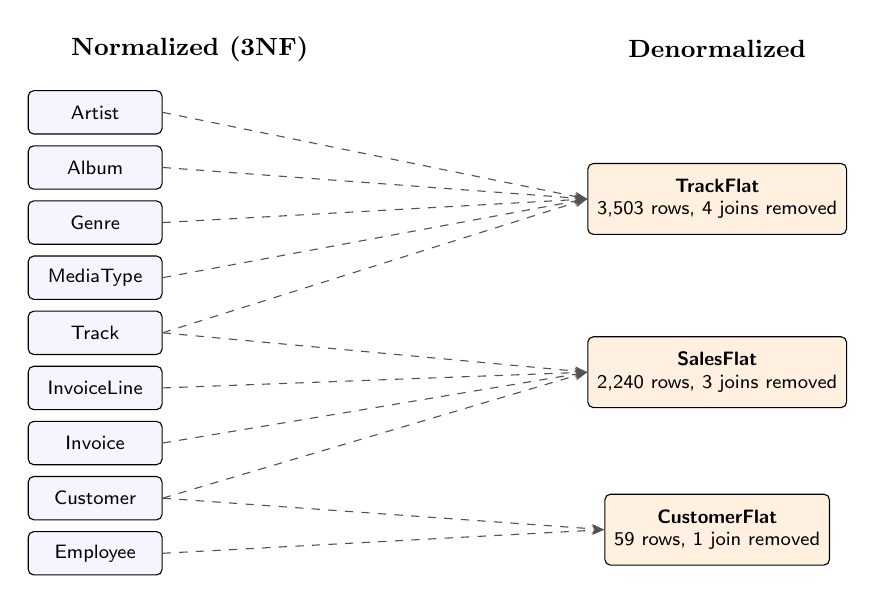
\begin{tikzpicture}[
  base/.style={draw, rounded corners=2pt, font=\scriptsize\sffamily, fill=blue!4,
               minimum width=17mm, minimum height=5.5mm},
  flat/.style={draw, rounded corners=2pt, font=\scriptsize\sffamily, fill=orange!12,
               minimum width=26mm, minimum height=9mm, align=center},
  absorb/.style={-{Stealth[length=1.6mm]}, dashed, gray!65!black, thin}
]
\node[font=\small\bfseries] at (-2.1,4.3) {Normalized (3NF)};
\node[font=\small\bfseries] at (4.6,4.3) {Denormalized};

\node[base] (artist)  at (-3.3,3.5) {Artist};
\node[base] (album)   at (-3.3,2.8) {Album};
\node[base] (genre)   at (-3.3,2.1) {Genre};
\node[base] (media)   at (-3.3,1.4) {MediaType};
\node[base] (track)   at (-3.3,0.7) {Track};
\node[base] (invline) at (-3.3,0.0) {InvoiceLine};
\node[base] (invoice) at (-3.3,-0.7) {Invoice};
\node[base] (cust)    at (-3.3,-1.4) {Customer};
\node[base] (emp)     at (-3.3,-2.1) {Employee};

\node[flat] (tf) at (4.6,2.4)  {\textbf{TrackFlat}\\3,503 rows, 4 joins removed};
\node[flat] (sf) at (4.6,0.2)  {\textbf{SalesFlat}\\2,240 rows, 3 joins removed};
\node[flat] (cf) at (4.6,-1.8) {\textbf{CustomerFlat}\\59 rows, 1 join removed};

\foreach \n in {artist,album,genre,media,track} \draw[absorb] (\n.east) -- (tf.west);
\foreach \n in {invline,invoice,cust,track}     \draw[absorb] (\n.east) -- (sf.west);
\foreach \n in {cust,emp}                       \draw[absorb] (\n.east) -- (cf.west);
\end{tikzpicture}
\end{center}

\noindent
Dashed arrows show absorption: each flat table stores a pre-joined copy of the tables feeding
into it. \texttt{Track} and \texttt{Customer} each feed two flat tables, so their attributes are
duplicated twice over.

\subsection{Dependencies and normal forms violated}

\begin{center}
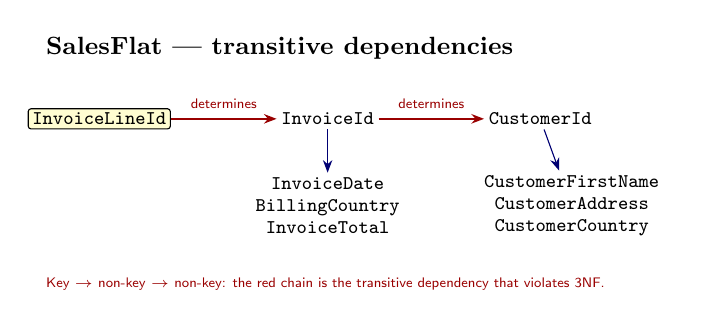
\begin{tikzpicture}[
  att/.style={font=\scriptsize\ttfamily, inner sep=1.5pt},
  key/.style={att, draw, fill=yellow!18, rounded corners=1pt},
  fd/.style={-{Stealth[length=1.6mm]}, blue!45!black},
  trans/.style={-{Stealth[length=1.6mm]}, red!60!black, thick}
]
\node[font=\small\bfseries, anchor=west] at (-0.4,1.5) {SalesFlat --- transitive dependencies};
\node[key] (k)  at (0.4,0.6)  {InvoiceLineId};
\node[att] (i)  at (3.3,0.6)  {InvoiceId};
\node[att] (c)  at (6.0,0.6)  {CustomerId};
\node[att] (ia) at (3.3,-0.5) {\parbox{2.6cm}{\centering InvoiceDate\\BillingCountry\\InvoiceTotal}};
\node[att] (ca) at (6.4,-0.5) {\parbox{2.8cm}{\centering CustomerFirstName\\CustomerAddress\\CustomerCountry}};

\draw[trans] (k)  -- node[above,font=\tiny\sffamily]{determines} (i);
\draw[trans] (i)  -- node[above,font=\tiny\sffamily]{determines} (c);
\draw[fd]    (i)  -- (ia);
\draw[fd]    (c)  -- (ca);
\node[font=\tiny\sffamily, text=red!60!black, anchor=west] at (-0.4,-1.5)
  {Key $\rightarrow$ non-key $\rightarrow$ non-key: the red chain is the transitive dependency
   that violates 3NF.};
\end{tikzpicture}
\end{center}


\paragraph{TrackFlat} (key \texttt{TrackId}). Since
$TrackId \rightarrow AlbumId$ and $AlbumId \rightarrow AlbumTitle,\,ArtistId$, the dependency
$TrackId \rightarrow AlbumTitle$ holds only transitively; likewise
$ArtistId \rightarrow ArtistName$, $GenreId \rightarrow GenreName$ and
$MediaTypeId \rightarrow MediaTypeName$. Non-key attributes thus depend on other non-key
attributes, \textbf{violating 3NF}. The table remains in 2NF, as a single-attribute key admits no
partial dependency. The redundancy is substantial: ``Iron Maiden'' is now stored 213 times and
``U2'' 135 times.

\paragraph{SalesFlat} (key \texttt{InvoiceLineId}). Two dependency chains hold:
\begin{align*}
InvoiceLineId &\rightarrow InvoiceId \\
InvoiceId &\rightarrow
  InvoiceDate,\; BillingCity,\; BillingCountry,\; InvoiceTotal,\; CustomerId \\
CustomerId &\rightarrow
  CustomerFirstName,\; CustomerLastName,\; CustomerAddress,\; CustomerCountry
\end{align*}
Both are transitive, again \textbf{violating 3NF}. An invoice with fourteen line items repeats
that customer's address fourteen times.

\paragraph{CustomerFlat} (key \texttt{CustomerId}). The chain
\[
CustomerId \rightarrow SupportRepId \rightarrow RepFirstName,\; RepLastName,\; RepTitle
\]
is a transitive dependency, \textbf{violating 3NF}. With 59 customers served by three
representatives, each representative's name is stored roughly twenty times.

\subsection{Anomalies introduced}

\begin{description}[leftmargin=*,style=nextline,topsep=2pt,itemsep=3pt]
  \item[Update anomaly] Correcting an artist's name requires updating every track row for that
    artist (213 rows for Iron Maiden) rather than one row in \texttt{Artist}. A partial update
    leaves two spellings of the same artist with no way to determine which is authoritative.
  \item[Insert anomaly] \texttt{TrackFlat} cannot record an artist or genre that has no tracks,
    and \texttt{SalesFlat} cannot record a customer who has never been invoiced, as there is no
    row in which to place them without fabricating a track or line item. Note that Q17 asks
    precisely about artists with no albums, so it still requires the normalized
    \texttt{Artist} table.
  \item[Delete anomaly] Deleting the final line item of an invoice erases that invoice's date and
    total; deleting an artist's last track erases the artist entirely.
  \item[Inconsistency risk] \texttt{CustomerCountry} and \texttt{BillingCountry} now coexist in
    \texttt{SalesFlat} and may disagree, with no constraint available to prevent it.
\end{description}

\subsection{Design decisions and cost}

\begin{itemize}[leftmargin=*,topsep=2pt,itemsep=3pt]
  \item Nullable foreign keys are flattened with \textsc{left join}. The present data contains no
    NULLs in those columns, but the schema permits them, and an \textsc{inner join} would
    silently drop rows, causing the denormalized copy to return different answers from the
    normalized one --- which would invalidate the Deliverable 2 timing comparison.
  \item \textbf{Verified equivalence.} Six representative queries (Q07, Q10, Q11, Q14, Q20) and
    all table row counts return identical results on both schemas. Any timing difference measured
    in Deliverable 2 is therefore attributable to schema design, not to differing answers.
  \item \textbf{Storage cost.} The database grows from 984\,KB to 1.7\,MB, approximately 73\%
    larger, for the same information content.
  \item The normalized tables are retained alongside the flat ones. That is itself a
    denormalization trade-off: duplicated storage in exchange for a join-free read path, which is
    the standard argument for a read-optimized reporting table.
\end{itemize}

\section{Evaluation pipeline design}\label{sec:pipeline}

The benchmark built above is the input to Deliverable 2. This section documents the architecture
we will execute against it, so that the design can be reviewed before the models are run.

\subsection{Component structure}

Each box is a module in \texttt{src/} with its public operations, drawn in UML class notation.
Dashed arrows are dependencies ($\langle\langle$use$\rangle\rangle$).

\begin{center}
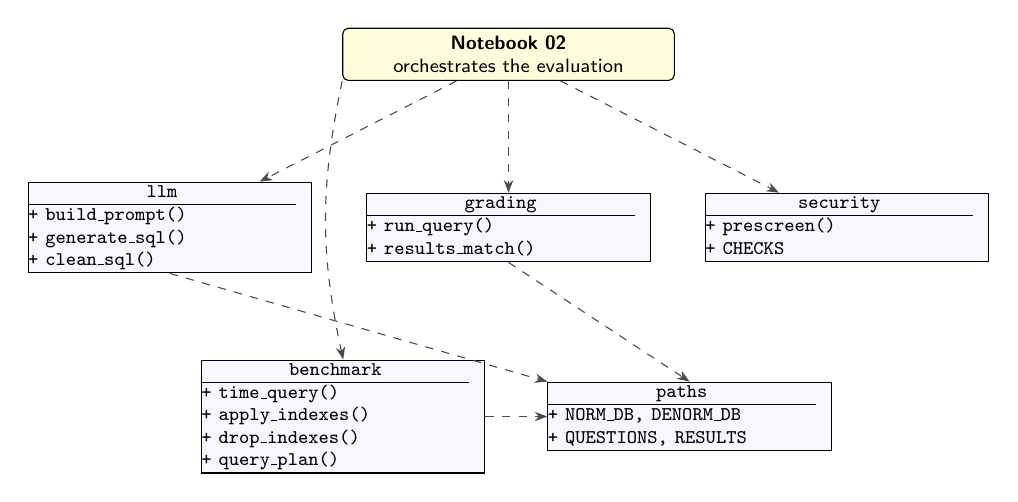
\begin{tikzpicture}[
  uml/.style={draw, font=\scriptsize\ttfamily, align=left, fill=blue!3, inner sep=0pt,
              text width=36mm},
  note/.style={draw, font=\scriptsize\sffamily, fill=yellow!14, align=center, rounded corners=2pt,
               text width=40mm, inner sep=3pt},
  use/.style={-{Stealth[length=1.6mm]}, dashed, gray!60!black}
]
\node[note] (nb) at (0,3.6) {\textbf{Notebook 02}\\\scriptsize orchestrates the evaluation};

\node[uml] (llm) at (-4.3,1.4) {%
  \begin{tabular}{@{}p{34mm}@{}}
  \multicolumn{1}{@{}c@{}}{\textbf{llm}}\\\hline
  + build\_prompt()\\
  + generate\_sql()\\
  + clean\_sql()\\\hline
  \end{tabular}};

\node[uml] (grade) at (0,1.4) {%
  \begin{tabular}{@{}p{34mm}@{}}
  \multicolumn{1}{@{}c@{}}{\textbf{grading}}\\\hline
  + run\_query()\\
  + results\_match()\\\hline
  \end{tabular}};

\node[uml] (sec) at (4.3,1.4) {%
  \begin{tabular}{@{}p{34mm}@{}}
  \multicolumn{1}{@{}c@{}}{\textbf{security}}\\\hline
  + prescreen()\\
  + CHECKS\\\hline
  \end{tabular}};

\node[uml] (bench) at (-2.1,-1.0) {%
  \begin{tabular}{@{}p{34mm}@{}}
  \multicolumn{1}{@{}c@{}}{\textbf{benchmark}}\\\hline
  + time\_query()\\
  + apply\_indexes()\\
  + drop\_indexes()\\
  + query\_plan()\\\hline
  \end{tabular}};

\node[uml] (paths) at (2.3,-1.0) {%
  \begin{tabular}{@{}p{34mm}@{}}
  \multicolumn{1}{@{}c@{}}{\textbf{paths}}\\\hline
  + NORM\_DB, DENORM\_DB\\
  + QUESTIONS, RESULTS\\\hline
  \end{tabular}};

\draw[use] (nb) -- (llm);
\draw[use] (nb) -- (grade);
\draw[use] (nb) -- (sec);
\draw[use] (nb.south west) to[bend right=12] (bench.north);
\draw[use] (llm.south) -- (paths.north west);
\draw[use] (grade.south) -- (paths.north);
\draw[use] (bench.east) -- (paths.west);
\end{tikzpicture}
\end{center}

\subsection{Sequence of one evaluated question}

\begin{center}
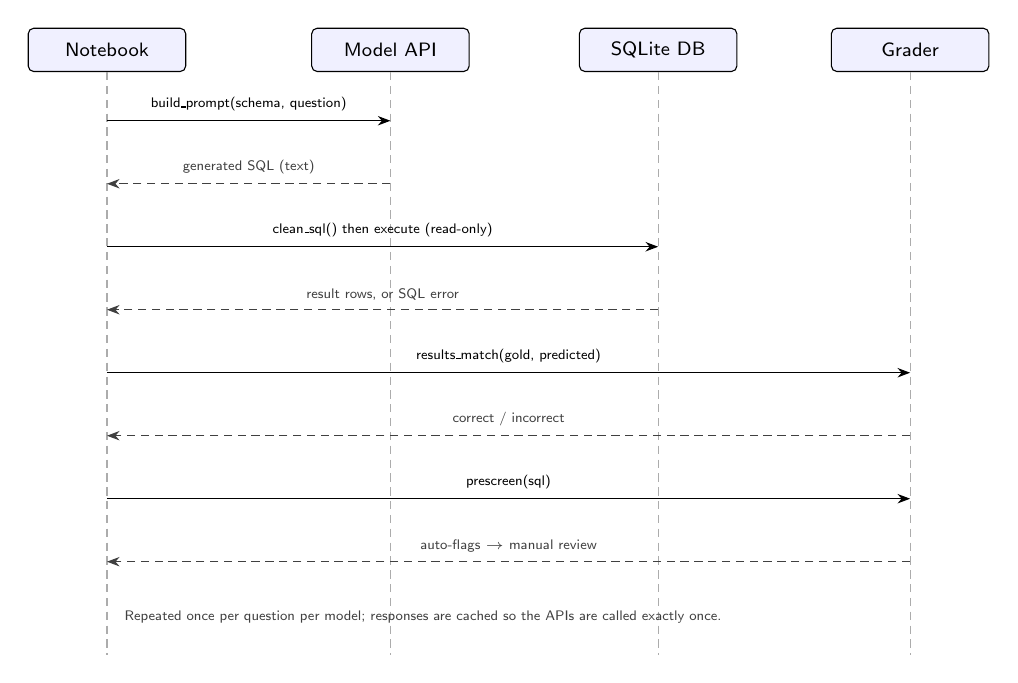
\begin{tikzpicture}[
  actor/.style={draw, rounded corners=2pt, font=\scriptsize\sffamily, fill=blue!6,
                minimum width=20mm, minimum height=5.5mm},
  life/.style={densely dashed, gray!65},
  msg/.style={-{Stealth[length=1.6mm]}, font=\tiny\sffamily},
  ret/.style={-{Stealth[length=1.6mm]}, densely dashed, font=\tiny\sffamily, gray!50!black}
]
\def\ytop{0}
\def\ybot{-7.4}
\node[actor] (n)  at (0,\ytop)   {Notebook};
\node[actor] (m)  at (3.6,\ytop) {Model API};
\node[actor] (d)  at (7.0,\ytop) {SQLite DB};
\node[actor] (g)  at (10.2,\ytop){Grader};
\foreach \n in {n,m,d,g} \draw[life] (\n.south) -- ++(0,\ybot);

\draw[msg] (0,-0.9)   -- node[above]{build\_prompt(schema, question)} (3.6,-0.9);
\draw[ret] (3.6,-1.7) -- node[above]{generated SQL (text)} (0,-1.7);
\draw[msg] (0,-2.5)   -- node[above]{clean\_sql() then execute (read-only)} (7.0,-2.5);
\draw[ret] (7.0,-3.3) -- node[above]{result rows, or SQL error} (0,-3.3);
\draw[msg] (0,-4.1)   -- node[above]{results\_match(gold, predicted)} (10.2,-4.1);
\draw[ret] (10.2,-4.9)-- node[above]{correct / incorrect} (0,-4.9);
\draw[msg] (0,-5.7)   -- node[above]{prescreen(sql)} (10.2,-5.7);
\draw[ret] (10.2,-6.5)-- node[above]{auto-flags $\rightarrow$ manual review} (0,-6.5);
\node[font=\tiny\sffamily, anchor=west, text=gray!50!black] at (0.1,-7.2)
  {Repeated once per question per model; responses are cached so the APIs are called exactly once.};
\end{tikzpicture}
\end{center}

\noindent
Correctness is decided on the \emph{result rows}, never on the SQL text, so a differently written
query that returns the same rows still counts as correct. Generated queries are executed through a
read-only connection, which is why a model's stray \texttt{DROP} or stacked statement is recorded
as a security flag rather than executed.

\subsection{Performance experiment}

\begin{center}
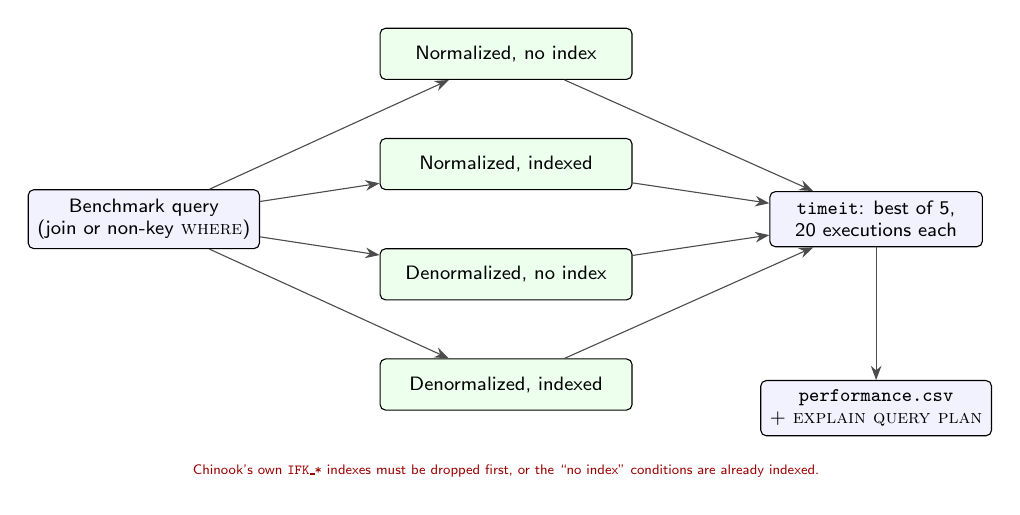
\begin{tikzpicture}[
  st/.style={draw, rounded corners=2pt, font=\scriptsize\sffamily, fill=blue!5, align=center,
             minimum height=7mm, minimum width=27mm},
  cond/.style={draw, rounded corners=2pt, font=\scriptsize\sffamily, fill=green!7, align=center,
               minimum height=6.5mm, minimum width=32mm},
  fl/.style={-{Stealth[length=1.8mm]}, gray!60!black}
]
\node[st] (q) at (0,0) {Benchmark query\\(join or non-key \textsc{where})};
\node[cond] (a) at (4.6,2.1)  {Normalized, no index};
\node[cond] (b) at (4.6,0.7)  {Normalized, indexed};
\node[cond] (c) at (4.6,-0.7) {Denormalized, no index};
\node[cond] (d) at (4.6,-2.1) {Denormalized, indexed};
\node[st] (t) at (9.3,0) {\texttt{timeit}: best of 5,\\20 executions each};
\node[st] (p) at (9.3,-2.4) {\texttt{performance.csv}\\+ \textsc{explain query plan}};
\foreach \n in {a,b,c,d} { \draw[fl] (q) -- (\n); \draw[fl] (\n) -- (t); }
\draw[fl] (t) -- (p);
\node[font=\tiny\sffamily, text=red!60!black, align=center] at (4.6,-3.2)
  {Chinook's own \texttt{IFK\_*} indexes must be dropped first, or the ``no index'' conditions are
   already indexed.};
\end{tikzpicture}
\end{center}

\section{Contribution statement}\label{sec:contrib}

This deliverable is submitted individually by each team member. The division of work below
reflects the commit history of the project repository as of \today.

\begin{description}[leftmargin=*,style=nextline,topsep=2pt,itemsep=3pt]
  \item[Jelani Denmark] Repository setup and the evaluation pipeline (prompting, result-set
    grading, security pre-screen, and timing modules); verification of all twenty gold queries
    against the database; the denormalized schema and its analysis (\S\ref{sec:denorm}); the
    Deliverable 2 benchmark queries, including the discovery that Chinook's built-in indexes
    invalidate a naive unindexed baseline; the ER and pipeline diagrams; and this document.
  \item[Joshua Sanders] Selection and adaptation of the twenty Spider questions, the gold SQL
    for the question set, and the question-sources and adaptations write-up
    (\S\ref{sec:questions}). Corrected three questions whose wording disagreed with their gold
    SQL following internal review.
  \item[Isaiah Washington] The relational algebra and tuple relational calculus queries
    (\S\ref{sec:algebra}), subsequently revised jointly to match the final question set.
  \item[Maxwell Amakor] Did not contribute.
\end{description}

\section{Known limitations}\label{sec:limits}

\begin{itemize}[leftmargin=*,topsep=2pt,itemsep=3pt]
  \item The question set contains easy and medium difficulty only, following the project guide's
    recommendation; no hard Spider questions are included.
  \item Q13 and Q14 use \textsc{order by \ldots\ limit 1}, which returns an arbitrary row when
    values tie. No ties exist in this data, and \S\ref{sec:algebra} documents the consequence.
  \item Q02 subtracts last names rather than customers, which yields the correct answer only
    because all 59 customers have distinct last names.
  \item Chinook ships 11 foreign-key indexes of its own. An initial timing run showed normalized
    queries gaining almost nothing from added indexes, because the ``unindexed'' baseline was in
    fact already using \texttt{IFK\_TrackGenreId}. The Deliverable 2 benchmark therefore drops
    and recreates Chinook's own indexes by name to obtain a genuinely unindexed baseline. We
    record this here because it affects the validity of any index comparison on this schema.
  \item The spelling errors inherited from Spider's question wording were retained deliberately
    (\S\ref{sec:questions}).
\end{itemize}

\appendix
\section{Normalized schema (DDL)}\label{app:ddl}

Generated from the live database by \texttt{scripts/setup\_db.py}; this is the exact text supplied
to both models in the Deliverable 2 prompt.

\lstinputlisting{generated/ddl.sql}

\section{Questions, gold SQL, and verified results}\label{app:questions}

% GENERATED by scripts/make_latex_appendices.py -- do not edit by hand.

\noindent Each entry gives the natural-language question as sent to the models, its
verified gold SQL, and the result that SQL returns against \texttt{data/chinook.db}.
Owner initials identify the team member who verified the answer.

\subsection*{Q01 --- Find the average unite price for a track.}

\begin{tabular}{@{}ll@{}}
\textbf{Difficulty} & easy \\
\textbf{Shape} & lookup \\
\textbf{Source} & chinnok\_1, train\_spider.json index 830 \\
\textbf{Verified by} & JD \\
\textbf{Row order matters} & no \\
\end{tabular}

\begin{lstlisting}
SELECT AVG(UnitPrice) FROM Track
\end{lstlisting}

\noindent\textbf{Result} (1 row): (1.051)

\subsection*{Q02 --- Find all the customer last names that do nout have invoice totals larger than 20.}

\begin{tabular}{@{}ll@{}}
\textbf{Difficulty} & medium \\
\textbf{Shape} & lookup \\
\textbf{Source} & chinnok\_1, train\_spider.json index 857 \\
\textbf{Verified by} & IW \\
\textbf{Row order matters} & no \\
\end{tabular}

\begin{lstlisting}
SELECT LastName FROM CUSTOMER EXCEPT SELECT T1.LastName FROM CUSTOMER AS T1 JOIN Invoice AS T2 ON T1.CustomerId  =  T2.CustomerId WHERE T2.total  >  20
\end{lstlisting}

\noindent\textbf{Result} (55 rows): (Almeida), (Barnett), (Bernard), (Brooks), (Brown), (Chase), (Dubois), (Fernandes), (Francis), (Girard), (Gonçalves), (Gordon), (Goyer), (Gray), (Gruber), (Gutiérrez), (Hansen), (Harris), (Hughes), (Hämäläinen), \ldots

\subsection*{Q03 --- What are the distinct billing countries of the invoices?}

\begin{tabular}{@{}ll@{}}
\textbf{Difficulty} & easy \\
\textbf{Shape} & lookup \\
\textbf{Source} & chinnok\_1, train\_spider.json index 815 \\
\textbf{Verified by} & MA \\
\textbf{Row order matters} & no \\
\end{tabular}

\begin{lstlisting}
SELECT DISTINCT BILLINGCOUNTRY FROM INVOICE
\end{lstlisting}

\noindent\textbf{Result} (24 rows): (Germany), (Norway), (Belgium), (Canada), (USA), (France), (Ireland), (United Kingdom), (Australia), (Chile), (India), (Brazil), (Portugal), (Netherlands), (Spain), (Sweden), (Czech Republic), (Finland), (Denmark), \ldots

\subsection*{Q04 --- How many distinct cities does the employee live in?}

\begin{tabular}{@{}ll@{}}
\textbf{Difficulty} & easy \\
\textbf{Shape} & lookup \\
\textbf{Source} & chinnok\_1, train\_spider.json index 853 \\
\textbf{Verified by} & JS \\
\textbf{Row order matters} & no \\
\end{tabular}

\begin{lstlisting}
SELECT COUNT(DISTINCT city) FROM EMPLOYEE
\end{lstlisting}

\noindent\textbf{Result} (1 row): (3)

\subsection*{Q05 --- List the phone numbers of all employees.}

\begin{tabular}{@{}ll@{}}
\textbf{Difficulty} & easy \\
\textbf{Shape} & lookup \\
\textbf{Source} & chinnok\_1, train\_spider.json index 864 \\
\textbf{Verified by} & JD \\
\textbf{Row order matters} & no \\
\end{tabular}

\begin{lstlisting}
SELECT Phone FROM EMPLOYEE
\end{lstlisting}

\noindent\textbf{Result} (8 rows): (+1 (780) 428-9482), (+1 (403) 262-3443), (+1 (403) 262-3443), (+1 (403) 263-4423), (1 (780) 836-9987), (+1 (403) 246-9887), (+1 (403) 456-9986), (+1 (403) 467-3351)

\subsection*{Q06 --- What are the invoice dates for customers with the first name Astrid and the last name Gruber?}

\begin{tabular}{@{}ll@{}}
\textbf{Difficulty} & medium \\
\textbf{Shape} & join \\
\textbf{Source} & chinnok\_1, train\_spider.json index 856 \\
\textbf{Verified by} & IW \\
\textbf{Row order matters} & no \\
\end{tabular}

\begin{lstlisting}
SELECT T2.InvoiceDate FROM CUSTOMER AS T1 JOIN INVOICE AS T2 ON T1.CustomerId = T2.CustomerId  WHERE T1.FirstName ='Astrid' AND T1.LastName = 'Gruber'
\end{lstlisting}

\noindent\textbf{Result} (7 rows): (2021-12-08 00:00:00), (2022-01-18 00:00:00), (2022-09-18 00:00:00), (2024-04-24 00:00:00), (2024-07-27 00:00:00), (2024-10-29 00:00:00), (2025-06-19 00:00:00)

\subsection*{Q07 --- What are the addresses of customers living in Germany who have had an invoice?}

\begin{tabular}{@{}ll@{}}
\textbf{Difficulty} & medium \\
\textbf{Shape} & join \\
\textbf{Source} & chinnok\_1, train\_spider.json index 862 \\
\textbf{Verified by} & MA \\
\textbf{Row order matters} & no \\
\end{tabular}

\begin{lstlisting}
SELECT DISTINCT T1.Address FROM CUSTOMER AS T1 JOIN INVOICE AS T2 ON T1.CustomerId = T2.CustomerId WHERE T1.Country = 'Germany'
\end{lstlisting}

\noindent\textbf{Result} (4 rows): (Theodor-Heuss-Straße 34), (Tauentzienstraße 8), (Berger Straße 10), (Barbarossastraße 19)

\subsection*{Q08 --- Find the number of albums by that artist Metallica}

\begin{tabular}{@{}ll@{}}
\textbf{Difficulty} & medium \\
\textbf{Shape} & join \\
\textbf{Source} & chinnok\_1, chinook\_1, train\_spider.json index 822 \\
\textbf{Verified by} & JS \\
\textbf{Row order matters} & no \\
\end{tabular}

\begin{lstlisting}
SELECT COUNT(*) FROM ALBUM AS T1 JOIN ARTIST AS T2 ON T1.ArtistId = T2.ArtistId WHERE T2.Name = 'Metallica'
\end{lstlisting}

\noindent\textbf{Result} (1 row): (10)

\subsection*{Q09 --- What are the duration of the longest and shortest pop tracks in milliseconds?}

\begin{tabular}{@{}ll@{}}
\textbf{Difficulty} & medium \\
\textbf{Shape} & join \\
\textbf{Source} & chinnok\_1, train\_spider.json index 881 \\
\textbf{Verified by} & JD \\
\textbf{Row order matters} & no \\
\end{tabular}

\begin{lstlisting}
SELECT MAX(T2.Milliseconds), MIN(T2.Milliseconds) FROM GENRE AS T1 JOIN TRACK AS T2 ON T1.GenreId = T2.GenreId WHERE T1.Name = 'Pop';
\end{lstlisting}

\noindent\textbf{Result} (1 row): (663426, 129666)

\subsection*{Q10 --- Count the number of tracks that are of the media type 'AAC audio file'.}

\begin{tabular}{@{}ll@{}}
\textbf{Difficulty} & medium \\
\textbf{Shape} & join \\
\textbf{Source} & chinnok\_1, train\_spider.json index 866 \\
\textbf{Verified by} & IW \\
\textbf{Row order matters} & no \\
\end{tabular}

\begin{lstlisting}
SELECT COUNT(*) FROM MEDIATYPE AS T1 JOIN TRACK AS T2 ON T1.MediaTypeId = T2.MediaTypeId WHERE T1.Name = 'AAC audio file';
\end{lstlisting}

\noindent\textbf{Result} (1 row): (11)

\subsection*{Q11 --- What is the first name and last name employee helps the customer with first name Leonie?}

\begin{tabular}{@{}ll@{}}
\textbf{Difficulty} & medium \\
\textbf{Shape} & join \\
\textbf{Source} & chinnok\_1, train\_spider.json index 849 \\
\textbf{Verified by} & MA \\
\textbf{Row order matters} & no \\
\end{tabular}

\begin{lstlisting}
SELECT T2.FirstName, T2.LastName FROM CUSTOMER AS T1 JOIN EMPLOYEE AS T2 ON T1.SupportRepId = T2.EmployeeId WHERE T1.FirstName = 'Leonie';
\end{lstlisting}

\noindent\textbf{Result} (1 row): (Steve, Johnson)

\noindent\textbf{Adaptation}: none needed chinook uses identical table/column names

\subsection*{Q12 --- What are the first names and support rep ids for employees serving 10 or more customers?}

\begin{tabular}{@{}ll@{}}
\textbf{Difficulty} & medium \\
\textbf{Shape} & aggregation \\
\textbf{Source} & chinnok\_1, train\_spider.json index 870 \\
\textbf{Verified by} & JS \\
\textbf{Row order matters} & no \\
\end{tabular}

\begin{lstlisting}
SELECT T2.FirstName, T1.SupportRepId FROM CUSTOMER AS T1 JOIN EMPLOYEE AS T2 ON T1.SupportRepId = T2.EmployeeId GROUP BY T1.SupportRepId, T2.FirstName HAVING COUNT(*) >= 10;
\end{lstlisting}

\noindent\textbf{Result} (3 rows): (Jane, 3), (Margaret, 4), (Steve, 5)

\noindent\textbf{Adaptation}: corrected original gold SQL it selected customer's firstName instead of employee's and wasn't grouped correctly

\subsection*{Q13 --- What is the least commone media type in all tracks?}

\begin{tabular}{@{}ll@{}}
\textbf{Difficulty} & medium \\
\textbf{Shape} & aggregation \\
\textbf{Source} & chinnok\_1, train\_spider.json index 837 \\
\textbf{Verified by} & JD \\
\textbf{Row order matters} & yes \\
\end{tabular}

\begin{lstlisting}
SELECT T1.Name FROM MEDIATYPE AS T1 JOIN TRACK AS T2 ON T1.MediaTypeId = T2.MediaTypeId GROUP BY T1.Name ORDER BY COUNT(*) ASC LIMIT 1;
\end{lstlisting}

\noindent\textbf{Result} (1 row): (Purchased AAC audio file)

\noindent\textbf{Adaptation}: tightened the GROUP BY to include both MediaTypeId and Name for correctness

\subsection*{Q14 --- Which artist has the most albums?}

\begin{tabular}{@{}ll@{}}
\textbf{Difficulty} & medium \\
\textbf{Shape} & aggregation \\
\textbf{Source} & chinnok\_1, train\_spider.json index 825 \\
\textbf{Verified by} & IW \\
\textbf{Row order matters} & yes \\
\end{tabular}

\begin{lstlisting}
SELECT T2.NAME FROM ALBUM AS T1 JOIN ARTIST AS T2 ON T1.ArtistId = T2.ArtistId GROUP BY T2.Name ORDER BY COUNT(*) DESC LIMIT 1;
\end{lstlisting}

\noindent\textbf{Result} (1 row): (Iron Maiden)

\subsection*{Q15 --- What are the titles and ids for albums containing tracks with unit price greater than 1?}

\begin{tabular}{@{}ll@{}}
\textbf{Difficulty} & medium \\
\textbf{Shape} & aggregation \\
\textbf{Source} & chinnok\_1, train\_spider.json index 840 \\
\textbf{Verified by} & MA \\
\textbf{Row order matters} & no \\
\end{tabular}

\begin{lstlisting}
SELECT T1.Title, T2.AlbumId FROM ALBUM AS T1 JOIN TRACK AS T2 ON T1.AlbumId = T2.AlbumId WHERE T2.UnitPrice > 1 GROUP BY T2.AlbumId, T1.Title;
\end{lstlisting}

\noindent\textbf{Result} (12 rows): (Battlestar Galactica: The Story So Far, 226), (Battlestar Galactica, Season 3, 227), (Heroes, Season 1, 228), (Lost, Season 3, 229), (Lost, Season 1, 230), (Lost, Season 2, 231), \ldots

\noindent\textbf{Adaptation}: added Title to the GROUP BY for correctness

\subsection*{Q16 --- What are the last names of employees who serve at most 20 customers, including employees who serve no customers?}

\begin{tabular}{@{}ll@{}}
\textbf{Difficulty} & medium \\
\textbf{Shape} & aggregation \\
\textbf{Source} & chinnok\_1, train\_spider.json index 872 \\
\textbf{Verified by} & JS \\
\textbf{Row order matters} & no \\
\end{tabular}

\begin{lstlisting}
SELECT T2.LastName FROM EMPLOYEE AS T2 LEFT JOIN CUSTOMER AS T1 ON T1.SupportRepId = T2.EmployeeId GROUP BY T2.EmployeeId, T2.LastName HAVING COUNT(T1.CustomerId) <= 20;
\end{lstlisting}

\noindent\textbf{Result} (7 rows): (Adams), (Edwards), (Park), (Johnson), (Mitchell), (King), (Callahan)

\noindent\textbf{Adaptation}: corrected original gold SQL it selected customer's LastName instead of the employee's,

\subsection*{Q17 --- Count the number of artists who have not realeased an album?}

\begin{tabular}{@{}ll@{}}
\textbf{Difficulty} & medium \\
\textbf{Shape} & subquery \\
\textbf{Source} & chinnok\_1, train\_spider.json index 888 \\
\textbf{Verified by} & JD \\
\textbf{Row order matters} & no \\
\end{tabular}

\begin{lstlisting}
SELECT COUNT(*) FROM ARTIST AS T1 WHERE NOT EXISTS (SELECT 1 FROM ALBUM AS T2 WHERE T2.ArtistId = T1.ArtistId);
\end{lstlisting}

\noindent\textbf{Result} (1 row): (71)

\noindent\textbf{Adaptation}: used NOT EXISTS instead of original NOT IN for NULL

\subsection*{Q18 --- How many albums are there?}

\begin{tabular}{@{}ll@{}}
\textbf{Difficulty} & easy \\
\textbf{Shape} & lookup \\
\textbf{Source} & chinnok\_1, train\_spider.json index 807 \\
\textbf{Verified by} & IW \\
\textbf{Row order matters} & no \\
\end{tabular}

\begin{lstlisting}
SELECT COUNT(*) FROM ALBUM
\end{lstlisting}

\noindent\textbf{Result} (1 row): (347)

\noindent\textbf{Adaptation}: none needed chinook uses identical table/column names

\subsection*{Q19 --- How many customers have email that contains 'gmail.com'?}

\begin{tabular}{@{}ll@{}}
\textbf{Difficulty} & easy \\
\textbf{Shape} & lookup \\
\textbf{Source} & chinnok\_1, train\_spider.json index 847 \\
\textbf{Verified by} & MA \\
\textbf{Row order matters} & no \\
\end{tabular}

\begin{lstlisting}
SELECT COUNT(*) FROM CUSTOMER WHERE Email LIKE '%gmail.com%'
\end{lstlisting}

\noindent\textbf{Result} (1 row): (8)

\noindent\textbf{Adaptation}: none needed chinook uses identical table/column names

\subsection*{Q20 --- What is the average unit price of tracks that billing to Jazz genre?}

\begin{tabular}{@{}ll@{}}
\textbf{Difficulty} & medium \\
\textbf{Shape} & join \\
\textbf{Source} & chinnok\_1, train\_spider.json index 843 \\
\textbf{Verified by} & JS \\
\textbf{Row order matters} & no \\
\end{tabular}

\begin{lstlisting}
SELECT AVG(UnitPrice) FROM GENRE AS T1 JOIN TRACK AS T2 ON T1.GenreId = T2.GenreId WHERE T1.Name = 'Jazz';
\end{lstlisting}

\noindent\textbf{Result} (1 row): (0.99)

\noindent\textbf{Adaptation}: none needed chinook uses identical table/column names


\end{document}
